\documentclass[12pt,t]{beamer}
\usepackage{graphicx}
\setbeameroption{hide notes}
\setbeamertemplate{note page}[plain]
\usepackage{listings}

% get rid of junk
\usetheme{default}
\beamertemplatenavigationsymbolsempty
\hypersetup{pdfpagemode=UseNone} % don't show bookmarks on initial view


% font
\usepackage{fontspec}
\setsansfont
  [ ExternalLocation = Stuff/fonts/ ,
    UprightFont = *-regular ,
    BoldFont = *-bold ,
    ItalicFont = *-italic ,
    BoldItalicFont = *-bolditalic ]{texgyreheros}
\setbeamerfont{note page}{family*=pplx,size=\footnotesize} % Palatino for notes
% "TeX Gyre Heros can be used as a replacement for Helvetica"
% I've placed them in ../fonts/; alternatively you can install them
% permanently on your system as follows:
%     Download http://www.gust.org.pl/projects/e-foundry/tex-gyre/heros/qhv2.004otf.zip
%     In Unix, unzip it into ~/.fonts
%     In Mac, unzip it, double-click the .otf files, and install using "FontBook"

% named colors
\definecolor{offwhite}{RGB}{255,250,240}
\definecolor{gray}{RGB}{155,155,155}

\definecolor{background}{RGB}{255,255,255}
\definecolor{foreground}{RGB}{24,24,24}
\definecolor{title}{RGB}{27,94,134}
\definecolor{subtitle}{RGB}{22,175,124}
\definecolor{hilit}{RGB}{122,0,128}
\definecolor{vhilit}{RGB}{255,0,128}
\definecolor{lolit}{RGB}{100,100,100}

\definecolor{nhilit}{RGB}{128,0,128}  % hilit color in notes
\definecolor{nvhilit}{RGB}{255,0,128} % vhilit for notes

\newcommand{\hilit}{\color{hilit}}
\newcommand{\vhilit}{\color{vhilit}}
\newcommand{\nhilit}{\color{nhilit}}
\newcommand{\nvhilit}{\color{nvhilit}}
\newcommand{\lolit}{\color{lolit}}
\newcommand{\ticolor}{\color{title}}

% use those colors
\setbeamercolor{titlelike}{fg=title}
\setbeamercolor{subtitle}{fg=subtitle}
\setbeamercolor{institute}{fg=lolit}
\setbeamercolor{normal text}{fg=foreground,bg=background}
\setbeamercolor{item}{fg=foreground} % color of bullets
\setbeamercolor{subitem}{fg=lolit}
\setbeamercolor{itemize/enumerate subbody}{fg=lolit}
\setbeamertemplate{itemize subitem}{{\textendash}}
\setbeamerfont{itemize/enumerate subbody}{size=\footnotesize}
\setbeamerfont{itemize/enumerate subitem}{size=\footnotesize}

% page number
\setbeamertemplate{footline}{%
    \raisebox{5pt}{\makebox[\paperwidth]{\hfill\makebox[20pt]{\lolit
          \scriptsize\insertframenumber}}}\hspace*{5pt}}

% add a bit of space at the top of the notes page
\addtobeamertemplate{note page}{\setlength{\parskip}{12pt}}

% default link color
\hypersetup{colorlinks, urlcolor={hilit}}

\ifx\notescolors\undefined % slides
  % set up listing environment
  \lstset{language=bash,
          basicstyle=\ttfamily\scriptsize,
          frame=single,
          commentstyle=,
          backgroundcolor=\color{darkgray},
          showspaces=false,
          showstringspaces=false
          }
\else % notes
  \lstset{language=bash,
          basicstyle=\ttfamily\scriptsize,
          frame=single,
          commentstyle=,
          backgroundcolor=\color{offwhite},
          showspaces=false,
          showstringspaces=false
          }
\fi

% a few macros
\newcommand{\bi}{\begin{itemize}}
\newcommand{\bbi}{\vspace{24pt} \begin{itemize} \itemsep8pt}
\newcommand{\ei}{\end{itemize}}
\newcommand{\ig}{\includegraphics}
\newcommand{\subt}[1]{{\footnotesize \color{subtitle} {#1}}}
\newcommand{\ttsm}{\tt \small}
\newcommand{\ttfn}{\tt \footnotesize}
\newcommand{\figh}[2]{\centerline{\includegraphics[height=#2\textheight]{#1}}}
\newcommand{\figw}[2]{\centerline{\includegraphics[width=#2\textwidth]{#1}}}


%%%%%%%%%%%%%%%%%%%%%%%%%%%%%%%%%%%%%%%%%%%%%%%%%%%%%%%%%%%%%%%%%%%%%%
% end of header
%%%%%%%%%%%%%%%%%%%%%%%%%%%%%%%%%%%%%%%%%%%%%%%%%%%%%%%%%%%%%%%%%%%%%%

% title info
\title{Complex trait genetics in mice}
\author{Karl Broman}
\institute{Biostatistics \& Medical Informatics \\
  Univ.\ Wisconsin{\textendash}Madison}
\date{}



\begin{document}

% title slide
{
\setbeamertemplate{footline}{} % no page number here
\frame{
  \titlepage


{
\href{http://kbroman.org}{\tt \scriptsize \color{foreground} kbroman.org}
\\[-4pt]
\href{https://github.com/kbroman}{\tt \scriptsize \color{foreground} github.com/kbroman}
\\[-4pt]
\href{https://twitter.com/kwbroman}{\tt \scriptsize \color{foreground} @kwbroman}
\\[-3pt]
\scriptsize Slides: \href{http://bit.ly/BMI2017-03}{\tt \scriptsize
  \color{foreground} bit.ly/BMI2017-03}
}

\vspace{-7mm}
\hfill 
\includegraphics[height=6mm]{Figs/cc-zero.png}

}

\note{
  These are slides for a talk that I gave to prospective graduate
  students on 31 March 2017.

  The source for the slides is at GitHub:
  {\tt https://github.com/kbroman/Talk\_ProspStudents}

  Slides and interactive graphs: {\tt bit.ly/BMI2017-03}
}

}


\begin{frame}[c]{}

\vspace*{-1mm} \hspace*{-2mm}
\figw{Figs/inbredmice.jpg}{1.2}

\note{
I'll start with a bit of background.

I focus on genetics problems, and particularly on mouse genetics.

I think these are SWR mice; the photo is from David Threadgill.
}

\end{frame}



\begin{frame}{}

\vspace*{18mm}

\centerline{
\begin{minipage}[t]{50mm}
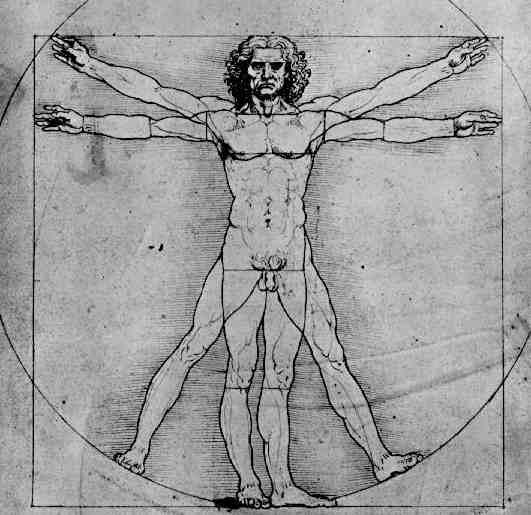
\includegraphics[height=50mm]{Figs/da-vinci-man.jpg}
\end{minipage}
\hspace{15mm}
\begin{minipage}[t]{50mm}
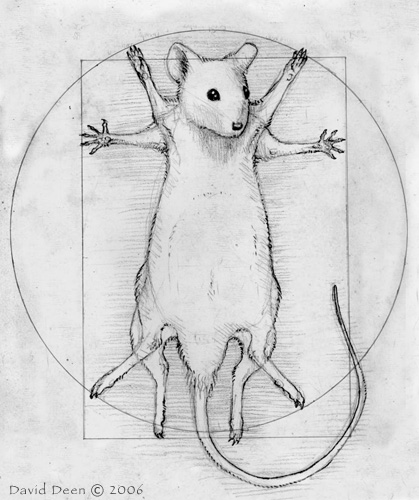
\includegraphics[height=50mm]{Figs/vitruvian_mouse.jpg}
\hspace{5mm}
\href{http://daviddeen.com}{\scriptsize \lolit \tt daviddeen.com}
\end{minipage}
}


\note{
Mice are not humans, but you can learn a great deal about human
biology and disease from mice.

The figure on the right is from David Deen.
}

\end{frame}


\begin{frame}[c]{Intercross}

\figh{Figs/intercross.pdf}{1.0}

\note{
  I've mostly focused on simple crosses between two inbred strains.

  Say strain P$_1$ has low blood pressure and P$_2$ has high blood
  pressure. We cross the two strains to get the F$_1$ hybrid, and then
  intercross F$_1$ siblings to get a large set of F$_2$
  individuals.

  The F$_2$ mice may inherit a P$_1$ or P$_2$ chromosome
  intact, but generally their chromosomes are a mosaic of the two
  parental chromosomes as a result of recombination at meiosis.  The
  points of exchange are called crossovers or recombination events.

  At any one autosomal locus, the F$_2$ individuals will have genotype
  BB, BR, or RR. We'd generate many such mice and then determine their
  genotype along chromosomes as well as measure their phenotype (e.g.,
  blood pressure). The simplest analyis is to look for genomic regions
  where genotype is associated with phenotype.
}
\end{frame}


\begin{frame}[c]{QTL mapping}

\vspace{5mm}
\only<1 | handout 0>{\figh{Figs/lodcurve_insulin.pdf}{0.9}}
\only<2>{\figh{Figs/lodcurve_insulin_with_effects.pdf}{0.9}}

\note{
  Our goal is to identify quantitative trait loci (QTL): regions of
  the genome for which genotype is associated with the phenotype.

  The basic analysis is to consider each locus, one at a time, split
  the mice into the three genotype groups, and perform analysis of
  variance.

  We then plot a test statistic that indicates the strength of the
  genotype-phenotype association.  For historical reasons, we
  calculate a LOD score as the test statistic: the log$_{10}$
  likelihood ratio comparing the hypothesis that there's a QTL at that
  position to the null hypothesis of no QTL anywhere.

  Large LOD scores indicate evidence for QTL and correspond to there
  being a difference in the phenotype average for the three genotype
  groups.
}
\end{frame}


\begin{frame}[c]{}

\figh{Figs/mouse_on_chips.png}{1.0}

\note{
I've mostly focused on a mapping genes affecting a single phenotype,
but in the past decade, I've become swamped with data.

This is a picture of a pile of gene expression arrays. More and more,
we're seeing genome-scale phenotype information. For example, in
one of my collaborations, we have data on 500 mice, each with gene
expression microarrays for 6 different tissues.

We're interested in identifying genes that control the expression of
other genes.
}

\end{frame}


\begin{frame}[c]{B6 $\times$ BTBR, \emph{Lep}$^{\text{\emph{ob}/\emph{ob}}}$}
\figh{Figs/plot-eqtl-islet.pdf}{0.9}

\note{
    In collaboration with Alan Attie, we've been studying
    a B6$\times$BTBR intercross, with all mice knocked out for leptin
    (and so obese), in order to understand obesity-induced diabetes.

    There are 500 intercross mice, phenotyped at a large number of
    clinical traits, and also with gene expression microarray data on
    6 tissues. These were custom two-color Agilent arrays.

    This figure shows the basic result of single-QTL genome scan for
    each expression trait, one at a time, in pancreatic islets. Each dot is
    an inferred QTL. The y-axis is the location of the corresponding
    microarray probe, and the x-axis is the location of the QTL.

    We see a prominent diagonal, of local-eQTL, and several prominent
    vertical bands: ``\emph{trans}-eQTL hotspots'' where genotype at a give
    region is associated with the mRNA expression of numerous genes across
    the genome.
}
\end{frame}



\begin{frame}[c]{B6 $\times$ BTBR, \emph{Lep}$^{\text{\emph{ob}/\emph{ob}}}$}
\figw{Figs/plot-eqtl.pdf}{1.1}

\note{
  Here are the results for all six tissues.

  There are numerous ``\emph{trans}-eQTL hotspots'' (where genotype at a give
  region is associated with the mRNA expression of numerous genes across
  the genome). Some of these \emph{trans}-eQTL hotspots are specific
  to a given tissue (e.g. islet chr 6) and some are seen in many
  tissues (e.g. chr 17).

  We seek to fine-map these \emph{trans}-eQTL hotspots, and to
  determine whether they involve one or multiple eQTL.
}

\end{frame}




\begin{frame}[c]{}

\large

\vspace*{10mm}
Slides: \href{http://bit.ly/BMI2017-03}{\tt bit.ly/BMI2017-03}

\vspace*{-5mm}
\hspace{90mm} 
\includegraphics[height=5mm]{Figs/cc-zero.png}

\vspace{2mm}

\href{http://kbroman.org}{\tt kbroman.org}

\vspace{2mm}

\href{https://github.com/kbroman}{\tt github.com/kbroman}

\vspace{2mm}

\href{https://twitter.com/kwbroman}{\tt @kwbroman}


\note{
  Here's where you can find me, as well as the slides for this talk.
}
\end{frame}

\end{document}
